\section{Задание 3. Прикладные задачи.}

\textbf{Условие.}

Решите задачи, следуя плану:
\begin{enumerate}
    \item Сделайте графическую иллюстрацию к задаче.
    \item Составьте математическую модель: введите обозначения, составьте формулу.
    \item Решите задачу аналитически.
    \item Запишите ответ.
\end{enumerate}

\begin{enumerate}
    \item Сторона квадрата увеличивается со скоростью $v$.
    Какова скорость изменения его периметра и площади в тот момент, когда сторона равна $a$?
    \item Проволокой длины $L$ необходимо огородить клумбу, имеющую форму кругового сектора.
    Найдите радиус круга, при котором площадь клумбы будет наибольшей.
\end{enumerate}
\vspace{10mm}
\textbf{Решение.}

\begin{enumerate}
    \item Введем обозначения: пусть $P(a) = 4a$ - периметр квадрата, а $S(a) = a^2$ - площадь квадрата,
    $v_a(t) = v$ - скорость увеличения квадрата в момент времени $t$ (аналогично $v_P(t)$ и $v_S(t)$ - скорости изменения периметра и площади)

    \begin{center}
        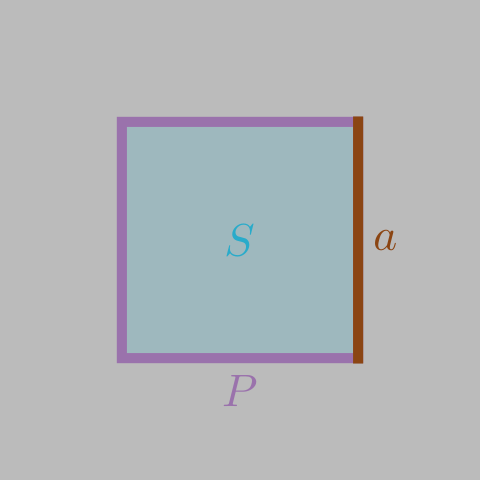
\includegraphics[width=10cm]{images/3a1}
    \end{center}

    Тогда:\\
    $\displaystyle a(t) = vt \qquad t = \frac{a}{v}\\
    P(t) = 4a(t) = 4vt\\
    S(t) = (a(t))^2 = v^2 t^2$

    Воспользуемся физическим смыслом производной:

    $\displaystyle v_P(t) = P^\prime(t) = 4v \quad v_P(a) = 4v\\
    v_S(t) = S^\prime(t) = 2 v^2 t \quad v_S(a) = 2 v^2 \frac{a}{v} = 2av$

    Получается, что в момент времени, когда сторона равна $a$, скорость увеличения периметра равна $4v$, и скорость увеличения площади равна $2av$

    \vspace{5mm}
    \textit{Ответ}: $4v$, $2av$

    \vspace{5mm}

    \item Введем обозначения: пусть $r$ - радиус сектора, $\varphi$ - угол сектора, а $S$ - площадь сектора.

    \begin{center}
        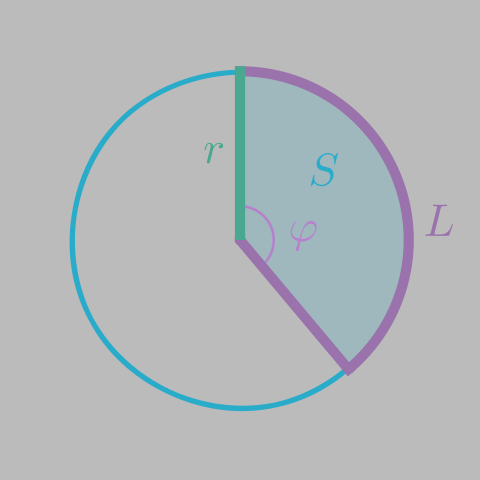
\includegraphics[width=10cm]{images/3b1}
    \end{center}

    Тогда: \\
    $\displaystyle
    L = 2r + 2\pi r \frac{\varphi}{2\pi} = 2r + \varphi r\\
    S = \pi r^2 \frac{\varphi}{2\pi} = \frac{\varphi r^2}{2}\\
    \varphi = \frac{L - 2r}{r} = \frac{L}{r} - 2\\
    S = \left(\frac{L}{r} - 2\right)\frac{r^2}{2} = \frac{Lr}{2} - r^2$ - площадь не зависит от угла сектора

    Найдем максимум функции $S(r)$:\\
    $\displaystyle S^\prime(r) = \frac{L}{2} - 2r\\
    S^\prime(r) = 0 \Longrightarrow r = \frac{L}{4}$

    При $\displaystyle r < \frac{L}{4}$ производная $S^\prime(r)$ больше нуля, а при $\displaystyle r > \frac{L}{4}$ меньше,
    поэтому в точке $\displaystyle r = \frac{L}{4}$ максимум функции, а, следовательно, площадь клумбы при $\displaystyle r = \frac{L}{4}$ наибольшая

    \vspace{5mm}
    \textit{Ответ}: $\displaystyle \frac{L}{4}$
\end{enumerate}


\clearpage
